% Farben für jede Schicht (\providecommand: auch im Skript definiert)
\providecommand{\applicationLayerColor}{Gold}
\providecommand{\transportLayerColor}{Indigo}
\providecommand{\networkLayerColor}{RoyalBlue}
\providecommand{\dataLinkLayerColor}{Gray}

% command to make sure colorboxes don't create whitespace between code lines
\fboxsep=.6pt

% default settings for listings
\lstset{style=python}

\title[Netzwerke]{Netzwerke}

\subtitle{Vermittlungsschicht (Skript, Abschnitt 1.4)}

\author[Blum, Cyril] % (optional)
{Cyril Blum}

\institute[KLW] % (optional)
{
    Fachschaft Informatik\\
    Kantonsschule im Lee
}

\date[\today] % (optional)

\logo{\includegraphics[width=2cm]{Logos/FreeFlower.pdf}}

\titlegraphic{\vspace{-.7cm}\includegraphics[width=.85\textwidth]{"Grundlagen_Info/06_Datenbanken/Figures/title-emojis"}}

\frame{\titlepage}

\section{Vermittlungsschicht}
\setbeamercolor{frametitle}{bg=\networkLayerColor!20}

\begin{frame}[fragile]{\faMapMarker{} \gls{IP}-Adresse}{Vermittlungsschicht}

    \begin{itemize}[<+->]
        \item \gls{IP}-Adresse = Netzwerk-Adresse eines Computers
        \item Analogie: Wohnadresse einer Person (Strasse \& Stadt)
        \item Häufig im \gls{IP}v4-Format: 4 bytes, also 4 Zahlen von 0-255, z.B.:\\
              \textcolor{blue}{\texttt{11000000.10101000.00000001.00000101}}
        \item Wird meist dezimal angegeben, z.B. \textcolor{blue}{\texttt{192.168.1.5}}

        \item Wie viele \gls{IP}v4-Adressen gibt es? Reicht das?
              \begin{itemize}
                  \item $4\cdot 8 \text{ bits} = 32 \text{ bits}$
                        \[2^{32} \sim 4 \text{ Milliarden Adressen} \rightarrow \text{zu wenig!}\]
              \end{itemize}
        \item \gls{IP}v6: 128 bits, fast unendlich viele Adressen
              \[2^{128} \sim 3.4\cdot 10^{38}  \text{ Adressen}\]
    \end{itemize}
\end{frame}

\begin{frame}{\faMapMarker{} \gls{IP}-Adresse}{Lokale und globale Adressen}
    \textbf{Lokale} vs. \textbf{globale} \gls{IP}-Adresse
    \begin{itemize}
        \item Aufgrund von \gls{IP}v4-Mangel: Unterscheidung zwischen lokalen und globalen \gls{IP}-Adressen
        \item \textbf{Lokale \gls{IP}}: nur im lokalen Netzwerk gültig (z.B. 192.168.x.x, 10.x.x.x)
        \item \textbf{Globale \gls{IP}}: weltweit eindeutig (z.B. 8.8.8.8)
    \end{itemize}
\end{frame}

\begin{frame}[fragile]{Lokale vs. globale \gls{IP}-Adresse}{\acrfull{NAT}}
    \begin{figure}[H]
        \centering
        \adjustbox{max width=\linewidth, max height=.55\textheight}{
            \begin{tikzpicture}[
                    base/.style={rectangle, draw, minimum width=2.5cm, minimum height=1cm, text=white, rounded corners, text width=2.5cm, align=center, inner sep=8pt},
                    device/.style={base, fill=ForestGreen},
                    router/.style={base, fill=\networkLayerColor},
                    server/.style={base, fill=Crimson},
                    arrow/.style={-Stealth, thick, text width=3cm, align=center}
                ]

                % Nodes
                \node[device] (client) {Client\\\texttt{192.168.0.10}};
                \node[device, below=.5cm of client] (client2) {Client\\\texttt{192.168.0.11}};
                \node[device, below=.5cm of client2] (client3) {Client\\\texttt{192.168.0.12}};
                \node[router, right=3cm of client2] (nat) {Router\\\texttt{80.152.43.21}};
                \node[server, right=3cm of nat] (web) {Webserver\\\texttt{159.233.1.22}};

                \node[draw=Crimson!60, rounded corners, thick, dashed, inner sep=6pt, fit=(client)(client2)(client3)(nat)] (lan2area){};

                % Label boxes
                \node[red, align=left, font=\small, anchor=south west] at (lan2area.north west) {Lokales Netzwerk};
                \node[below=0.5cm of web, text width=2.5cm, align=center, font=\small] {Internet};

                % Arrows and animations
                \only<1>{
                    \draw[arrow] (client.east) -- (nat.west) node[midway, above, text=black] {Anfrage von\\\texttt{192.168.0.10}};
                }

                \only<2>{
                    \draw[arrow] (nat.east) -- (web.west) node[midway, above, text=black] {Anfrage von\\\texttt{80.152.43.21} \faCheck};
                }

                \only<3>{
                    \draw[arrow] (web.west) -- (nat.east) node[midway, below, text=black] {Antwort an\\\texttt{80.152.43.21}};
                }

                \only<4>{
                    \draw[arrow] (nat.west) -- (client.east) node[midway, below, text=black] {Antwort an\\\texttt{192.168.0.10} \faCheck};
                }

                % NAT table
                \only<2->{
                    \node[below=0.1cm of nat, text width=3.5cm, font=\tiny, inner sep=8pt, draw, rounded corners, fill=\networkLayerColor!10] (natTable) {
                        \textbf{\acrshort{NAT}-Tabelle}
                        \begin{tabular}{p{1.4cm}p{1.4cm}}
                            \textbf{Lokal} & \textbf{Global} \\
                            \midrule
                            192.168.0.10 & 80.152.43.21 \\

                        \end{tabular}
                    };
                }
            \end{tikzpicture}
        }
    \end{figure}

    \only<1-2>{
        \textbf{Ausgehende Anfrage}
        \begin{itemize}
            \item Client sendet Anfrage mit lokaler \acrshort{IP}-Adresse
            \item Router ersetzt lokale \acrshort{IP} durch seine globale \acrshort{IP}
        \end{itemize}
    }

    \only<3-4>{
        \textbf{Eingehende Antwort}
        \begin{itemize}
            \item Server antwortet an die globale \acrshort{IP} des Routers
            \item Router schlägt in \acrshort{NAT}-Tabelle nach und leitet an lokale \acrshort{IP} weiter
        \end{itemize}
    }
\end{frame}

\begin{frame}[fragile]{Eigene \acrshort{IP}-Adresse herausfinden}
    \begin{itemize}
        \item MacOS, Terminal (via Spotlight-Suche): \\
              \commandbox*|ipconfig getifaddr en0|
        \item Windows, Programm \enquote{\texttt{cmd}} (via \keys{\faWindows + R}): \\
              \commandbox*|ipconfig|
    \end{itemize}
\end{frame}

\begin{frame}[fragile]{\faCompass{} \texttt{ping}}{Vermittlungsschicht}

    \begin{itemize}[<+->]
        \item Im Terminal / cmd: \commandbox*|ping [ip address]|, z.B.:\\
              \commandbox*|ping 159.233.1.22|
        \item Minimale Nachricht an andere \gls{IP}-Adresse schicken
        \item Ziel: schauen ob eine \gls{IP} existiert, bzw. erreichbar ist, wird mittels \gls{ICMP} realisiert
    \end{itemize}
\end{frame}

\begin{frame}[fragile]{Auftrag (Skript)}
    \begin{itemize}
        \item \aufgabebox{1.12: Eigene \acrshort{IP}v4-Adresse herausfinden}
        \item \challengebox{1.13: \texttt{ping} im echten Netzwerk testen}
        \item \challengebox{1.14 - 1.15: Python, \acrshort{ARP}-Scan}
        \item \aufgabebox{1.16 - 1.18: Notation \acrshort{IP}v4 und \acrshort{IP}v6}
        \item \aufgabebox{1.19 - 1.20: Gültige Adressen, grösste Adresse}
    \end{itemize}
\end{frame}

\begin{frame}[fragile]{\faMapMarker{} Sub-Netze}{Vermittlungsschicht}
    \begin{figure}[H]
        \centering
        \includegraphics[width=\linewidth, height=.75\textheight, keepaspectratio]{Grundlagen_Info/07_Netzwerke/Figures/subnets}
    \end{figure}
\end{frame}

\begin{frame}[fragile]{\faMapMarker{} Sub-Netze}{Vermittlungsschicht}
    \begin{center}
        \textbf{Switch} oder \textbf{Router}?!?
    \end{center}
    \begin{center}
        \resizebox{!}{.5\textheight}{% Typischer Heimrouter von vorne (neutral, ohne Marke): Gehäuse, Antennen, Status-LEDs.
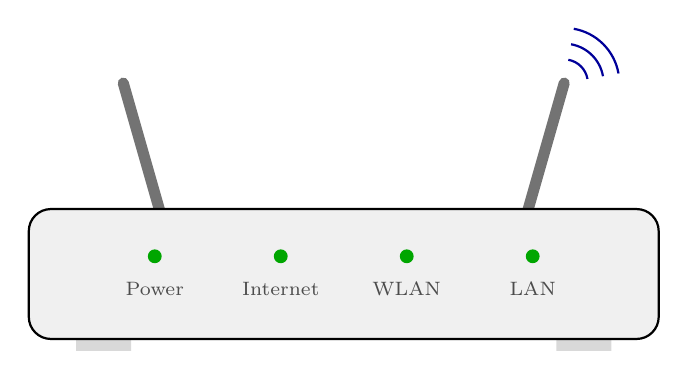
\begin{tikzpicture}[
        antenne/.style={line width=4pt, line cap=round, black!55},
        led/.style={circle, inner sep=0pt, minimum size=5pt, fill=green!65!black},
        ledtext/.style={font=\scriptsize, black!70, anchor=north}
    ]
    % Antennen hinter dem Gehäuse
    \draw[antenne] (-2.2,1.0) -- (-2.8,3.1);
    \draw[antenne] (2.2,1.0) -- (2.8,3.1);
    % Funkwellen
    \foreach \r in {0.3,0.5,0.7}
        \draw[blue!60!black, thick] (2.8,3.1) ++(10:\r) arc (10:80:\r);
    % Gehäuse
    \fill[black!15] (-3.4,-0.15) rectangle (-2.7,-0.3) (2.7,-0.15) rectangle (3.4,-0.3);
    \draw[thick, fill=black!6, rounded corners=8pt] (-4,-0.15) rectangle (4,1.5);
    % Status-LEDs
    \foreach \x/\t in {-2.4/Power, -0.8/Internet, 0.8/WLAN, 2.4/LAN} {
        \node[led] at (\x,0.9) {};
        \node[ledtext] at (\x,0.7) {\t};
    }
\end{tikzpicture}
}
    \end{center}
\end{frame}

\begin{frame}[fragile]{\faMapMarker{} Sub-Netze}{Vermittlungsschicht}
    \begin{center}
        \textbf{Switch} oder \textbf{Router}?!?
    \end{center}
    \begin{center}
        \resizebox{!}{.62\textheight}{% Heimrouter von hinten: Ab Overlay 2 wird sichtbar, welche Anschlüsse zu Router und Switch gehören.
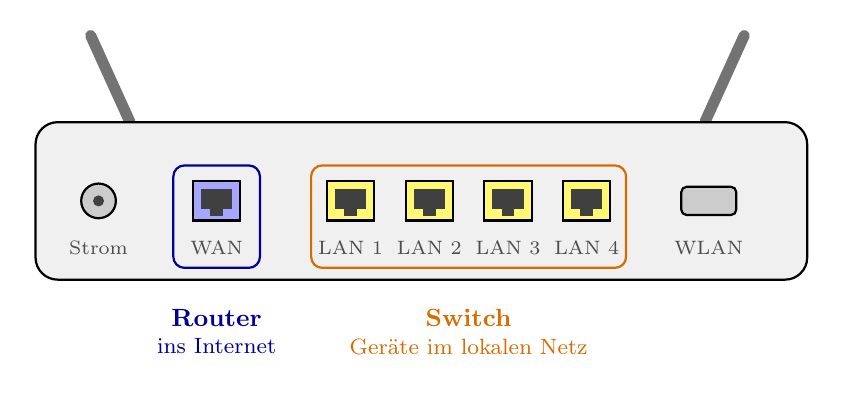
\begin{tikzpicture}[
        antenne/.style={line width=4pt, line cap=round, black!55},
        bereich/.style={draw, thick, rounded corners=4pt, inner sep=5pt},
        rolle/.style={font=\small\bfseries, align=center},
        portname/.style={font=\scriptsize, black!70},
        pics/rj45/.style={code={
            % Netzwerkbuchse: Rahmen mit Rastnase unten
            \draw[thick, fill=#1] (-0.3,-0.25) rectangle (0.3,0.25);
            \fill[black!75] (-0.2,0.15) rectangle (0.2,-0.1);
            \fill[black!75] (-0.08,-0.1) rectangle (0.08,-0.19);
        }}
    ]
    % Feste Grösse, damit die Folie beim Einblenden der Rollen nicht springt
    \useasboundingbox (-4.7,-2.4) rectangle (5.3,2.2);
    % Antennen
    \draw[antenne] (-3.4,1.0) -- (-3.9,2.1);
    \draw[antenne] (3.9,1.0) -- (4.4,2.1);
    % Gehäuse
    \draw[thick, fill=black!6, rounded corners=8pt] (-4.6,-1.0) rectangle (5.2,1.0);
    % Stromanschluss
    \draw[thick, fill=black!20] (-3.8,0) circle (0.22);
    \fill[black!75] (-3.8,0) circle (0.07);
    \node[portname] at (-3.8,-0.6) {Strom};
    % WAN-Anschluss
    \pic at (-2.3,0) {rj45=blue!35};
    \node[portname] at (-2.3,-0.6) {WAN};
    % Vier LAN-Anschlüsse
    \foreach \x/\n in {-0.6/1, 0.4/2, 1.4/3, 2.4/4} {
        \pic at (\x,0) {rj45=yellow!55};
        \node[portname] at (\x,-0.6) {LAN \n};
    }
    % WLAN-Taste
    \draw[thick, fill=black!20, rounded corners=2pt] (3.6,-0.18) rectangle (4.3,0.18);
    \node[portname] at (3.95,-0.6) {WLAN};
    % Rollen erst nach \pause auf der Folie einblenden
    \only<2->{
        \draw[bereich, blue!60!black] (-2.85,-0.85) rectangle (-1.75,0.45);
        \draw[bereich, orange!85!black] (-1.1,-0.85) rectangle (2.9,0.45);
        \node[rolle, blue!60!black, anchor=north] at (-2.3,-1.25) {Router\\[-1pt]\footnotesize\mdseries ins Internet};
        \node[rolle, orange!85!black, anchor=north] at (0.9,-1.25) {Switch\\[-1pt]\footnotesize\mdseries Geräte im lokalen Netz};
    }
\end{tikzpicture}
}
    \end{center}
    \pause
    \begin{center}
        Beides (meistens) im gleichen Gerät!
    \end{center}
\end{frame}

\begin{frame}[fragile]{\faMapMarker{} Sub-Netze}{Vermittlungsschicht}
    \textbf{Subnetzwerke}
    \begin{itemize}[<+->]
        \item Verschiedene Geräte gehören zum gleichen Subnetz, falls sie
              \begin{itemize}
                  \item physisch miteinander verbunden sind (\acrshort{WLAN}, Kabel, etc.)
                  \item denselben Netzwerkteil haben: \gls{IP}-Adressen stimmen überall dort überein, wo die Subnetzmaske eine 1 hat (später mehr dazu)
              \end{itemize}
    \end{itemize}
\end{frame}

\begin{frame}[fragile]{\faGlobe{} Netzmasken}{Vermittlungsschicht}
    \textbf{Netzmaske}
    \begin{itemize}[<+->]
        \item Sieht ähnlich aus wie eine \acrshort{IP}-Adresse: \commandBluebox|xxx.xxx.xxx.xxx|
        \item Fasst mehrere \acrshortpl{IP} zu einer Gruppe (= Subnetz) zusammen
        \item Gibt an, wie viele Stellen einer \acrshort{IP}-Adresse gleich sein müssen, damit mehrere Computer zum gleichen (Sub-)Netzwerk gehören.
        \item \textbf{Beispiel}:
              \begin{table}[H]
                  \centering
                  \tiny
                  \begin{tabular}{rll}
                                   & Dezimal                        & Binär                                                                 \\\midrule
                      \acrshort{IP} 1         & \texttt{159.233.1.22}          & \texttt{\textcolor{ForestGreen}{10011111.11101001.00000001}.00010110} \\\midrule
                      \acrshort{IP} 2         & \texttt{159.233.1.1}           & \texttt{\textcolor{ForestGreen}{10011111.11101001.00000001}.00000001} \\\midrule
                      Subnetzmaske & \commandBluebox|255.255.255.0| & \texttt{\textcolor{ForestGreen}{11111111.11111111.11111111}.00000000}
                  \end{tabular}
              \end{table}
              Bedeutet, dass alle \acrshort{IP}-Adressen die mit \commandbox|159.233.1.[...]| anfangen, zum selben Netzwerk gehören
        \item Wird manchmal \enquote{informell} auch so angegeben: \commandBluebox|159.233.1.x|
    \end{itemize}
\end{frame}

\begin{frame}[fragile]{Subnetze \& Netzmasken}{Übung}
    \begin{table}[H]
        \centering
        \footnotesize
        \begin{tabular}{lllp{2cm}}

            \textbf{Eigene \acrshort{IP}} & \textbf{Netzmaske} & \textbf{Ziel-\acrshort{IP}} & \textbf{Gleiches \newline Subnetz?} \\\midrule

            213.45.19.89       & 255.255.255.0      & 213.45.17.89     &                                     \\\midrule

            213.45.19.89       & 255.255.0.0        & 213.45.17.89     &                                     \\\midrule

            88.100.11.17       & 255.255.255.0      & 88.100.11.254    &                                     \\\midrule

            88.100.11.17       & 0.0.0.0            & 213.45.19.89     &                                     \\\midrule

            10.0.0.2           & 255.255.255.252    & 10.0.0.1         &                                     \\\midrule
            1.2.3.1            & 255.255.255.252    & 1.2.3.5          &
        \end{tabular}
    \end{table}
    \begin{itemize}
        \item $\rightarrow$ \acrshortpl{IP} dürfen sich nur an denjenigen Stellen unterscheiden, wo in der Maske (binär!) Nullen stehen.
        \item Umrechner dezimal $\rightarrow$ binär: \qrcode[height=1cm]{https://oinf.ch/interactive/ips-und-netzmaske/}
    \end{itemize}
\end{frame}

\begin{frame}[fragile]{Subnetze \& Netzmasken}{Aufträge (Skript)}
    \begin{itemize}
        \item Subnetzmasken
              \begin{itemize}
                  \item \aufgabebox{Netzmasken: 1.21-1.24}
                  \item \aufgabebox{Filius: 1.25}
                  \item \challengebox{1.26}
                  \item \aufgabebox{Filius: 1.27}
              \end{itemize}
    \end{itemize}
\end{frame}

\begin{frame}[fragile]{Subnetze \& Netzmasken}{Weitere Übungen (Lösung)}
    \begin{table}[H]
        \centering
        \adjustbox{max width=\textwidth, max totalheight=.8\textheight}{
            \begin{tabular}{p{1.2cm}cccccc}
                \textbf{Netzmaske Subnetz} & \multicolumn{2}{c}{255.255.255.0} & \multicolumn{2}{c}{255.255.0.0} & \multicolumn{2}{c}{255.255.255.240}                                        \\
                \cmidrule{2-7}
                                           & \acrshort{IP} 3.4.5.6                          & \acrshort{IP} 3.3.3.3                        & \acrshort{IP} 3.4.5.6                           & \acrshort{IP} 3.3.3.3 & \acrshort{IP} 3.4.5.6 & \acrshort{IP} 3.3.3.3 \\
                \midrule
                3.3.3.4                    & Nein                                & Ja                                & Nein                                 & Ja         & Nein       & Ja         \\\midrule
                4.4.4.3                    & Nein                                & Nein                              & Nein                                 & Nein       & Nein       & Nein       \\\midrule
                3.4.5.99                   & Ja                                  & Nein                              & Ja                                   & Nein       & Nein       & Nein       \\\midrule
                3.3.4.4                    & Nein                                & Nein                              & Nein                                 & Ja         & Nein       & Nein       \\\midrule
                3.4.7.7                    & Nein                                & Nein                              & Ja                                   & Nein       & Nein       & Nein       \\\midrule
                3.3.3.17                   & Nein                                & Ja                                & Nein                                 & Ja         & Nein       & Nein       \\
            \end{tabular}}
    \end{table}
\end{frame}

